\newcommand{\red}{\textcolor{red}{T1}}
\newcommand{\blue}{\textcolor{blue}{T4}}
\newcommand{\bluedrei}{\textcolor{blue}{T3}}
\newcommand{\tg}[1]{\textcolor{green}{#1}}
\newcommand{\tdg}[1]{\textcolor{darkgreen}{#1}}
\newcommand{\cen}{\textcolor{orange}{\textbf{c}}}
\newcommand{\reda}{\textcolor{red}{a}}
\newcommand{\blueb}{\textcolor{blue}{b}}

\fbox{
\begin{minipage}{0.2\textwidth}
\minpurp{Rotationen}
\quarterpage{
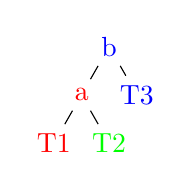
\begin{tikzpicture}[level distance=1.75em, sibling distance = 2em]
\node{ \blueb }
child{ node{\reda}
child{ node{\red}}
child{ node{\tg{T2}}}}
child{ node{\bluedrei}
}
;
\end{tikzpicture}}
\quarterpage{ \centering 
Rechts um \textcolor{red}{a} \\
$\Longrightarrow$ \\
Links um \textcolor{blue}{b} \\
$\Longleftarrow$
}
\quarterpage{
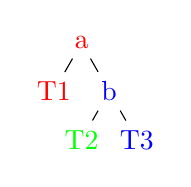
\begin{tikzpicture}[level distance=1.75em, sibling distance = 2em]
\node{\reda} 
child{ node{\red}}
child{node{\blueb}
child{ node{\tg{T2}}}
child{node{\bluedrei}}
};
\end{tikzpicture}}
\end{minipage}   \begin{minipage}{0.1pt}
\rule{0.5pt}{10em}
\end{minipage}\!     
\begin{minipage}{0.25\textwidth}{
\minpurp{Doppelrotation}
-2 \rule{10em}{0pt}  +2\\
\begin{minipage}[t]{0.25\textwidth} 
\begin{tikzpicture}[level distance=1.75em, sibling distance = 2em]
\node{\blueb} 
child{ node{\reda}
child{ node{\red}
}
child{ node{\cen}
child{ node{\tg{T2}}}
child{ node{\tdg{T3}}}
}
}
child{ node{\blue}}
;
\end{tikzpicture}\end{minipage}
\begin{minipage}[t]{0.35\textwidth}
\begin{tikzpicture}[sibling distance=3em, level distance=1.5em ,level 2/.style={sibling distance=1.5em} ]
\node{\cen}
  child{ node{\reda}{
    child{ node{\red}}
    child{ node{\tg{T2}}}
  }}
  child{ node{\blueb}
    child{ node{\tdg{T3}}}
    child{ node{\blue}}
  };
\end{tikzpicture}
\end{minipage} \rule{0.05pt}{7em}
\begin{minipage}[t]{0.22\textwidth}
\begin{tikzpicture}[level distance=1.75em, sibling distance = 2em]
\node(a){\reda} 
child{ node{\red}}
child{ node{\blueb}
child{ node{\cen}
child{ node{\tg{T2}}}
child{ node{\tdg{T3}}}}
child{ node{\blue}
}
}
;
\end{tikzpicture} 
\end{minipage}}\end{minipage}}